\section{Progettazione}
\label{sec:progettazione}
\subsection{Classi utilizzate}
\begin{figure}[h]
    \centering
    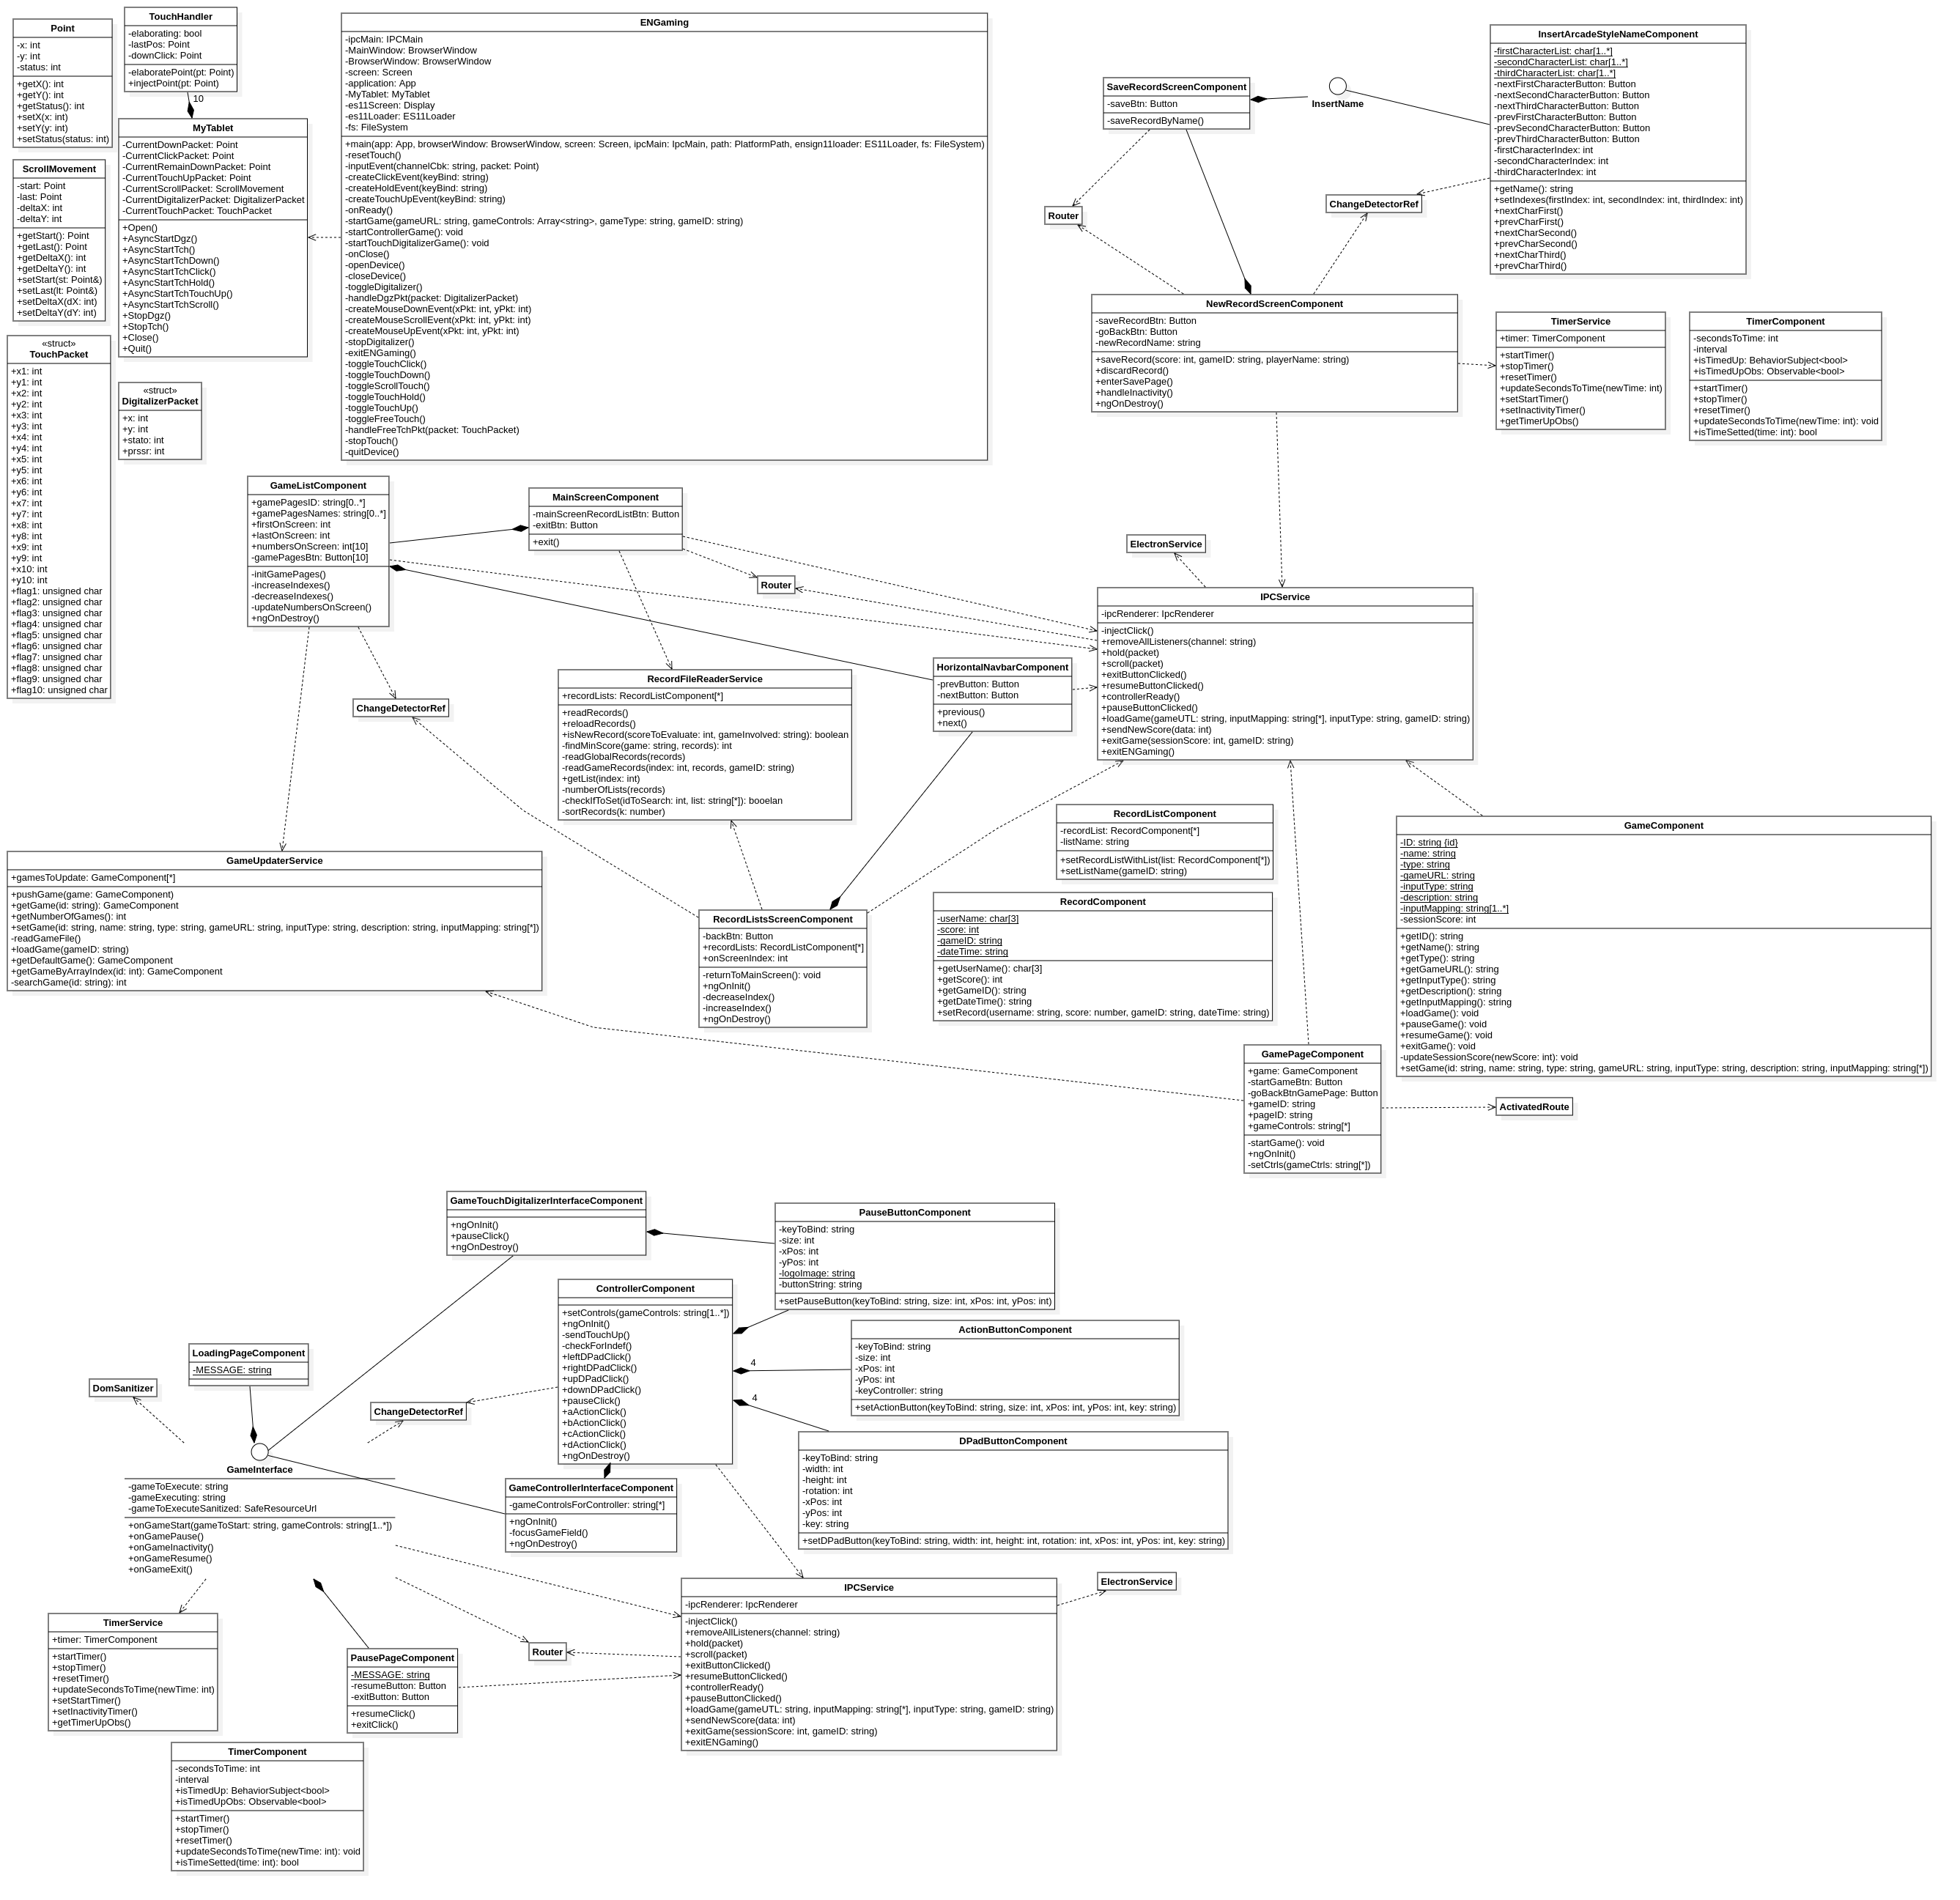
\includegraphics[width=340pt]{images/prog/ENGaming.png}
    \caption{Diagramma completo delle classi utilizzate}
    \label{fig:diagrammaCompleto}
\end{figure}
% immagine grafico completo
Le classi utilizzate possono essere classificate tramite il linguaggio di implementazione:
\begin{itemize}
    \item Electron: \begin{itemize}
        \item ENGaming
    \end{itemize}
    \item C++: \begin{itemize}
        \item MyTablet
        \item TouchHandler
        \item Point
        \item ScrollMovement
        \item TouchPacket
        \item DigitalizerPacket
    \end{itemize}
    \item Angular: \begin{itemize}
        \item Tutte le classi "Component"
        \item Tutte le classi "Service"
        \item GameInterface
        \item InsertName
        \item Router
        \item ChangeDetectorRef
        \item DomSanitizer
        \item ActivatedRoute
    \end{itemize}
\end{itemize}
Di seguito si analizzano le vari componenti con maggior dettaglio.
\newpage
\subsubsection{ENGaming}
\begin{figure}[h]
    \centering
    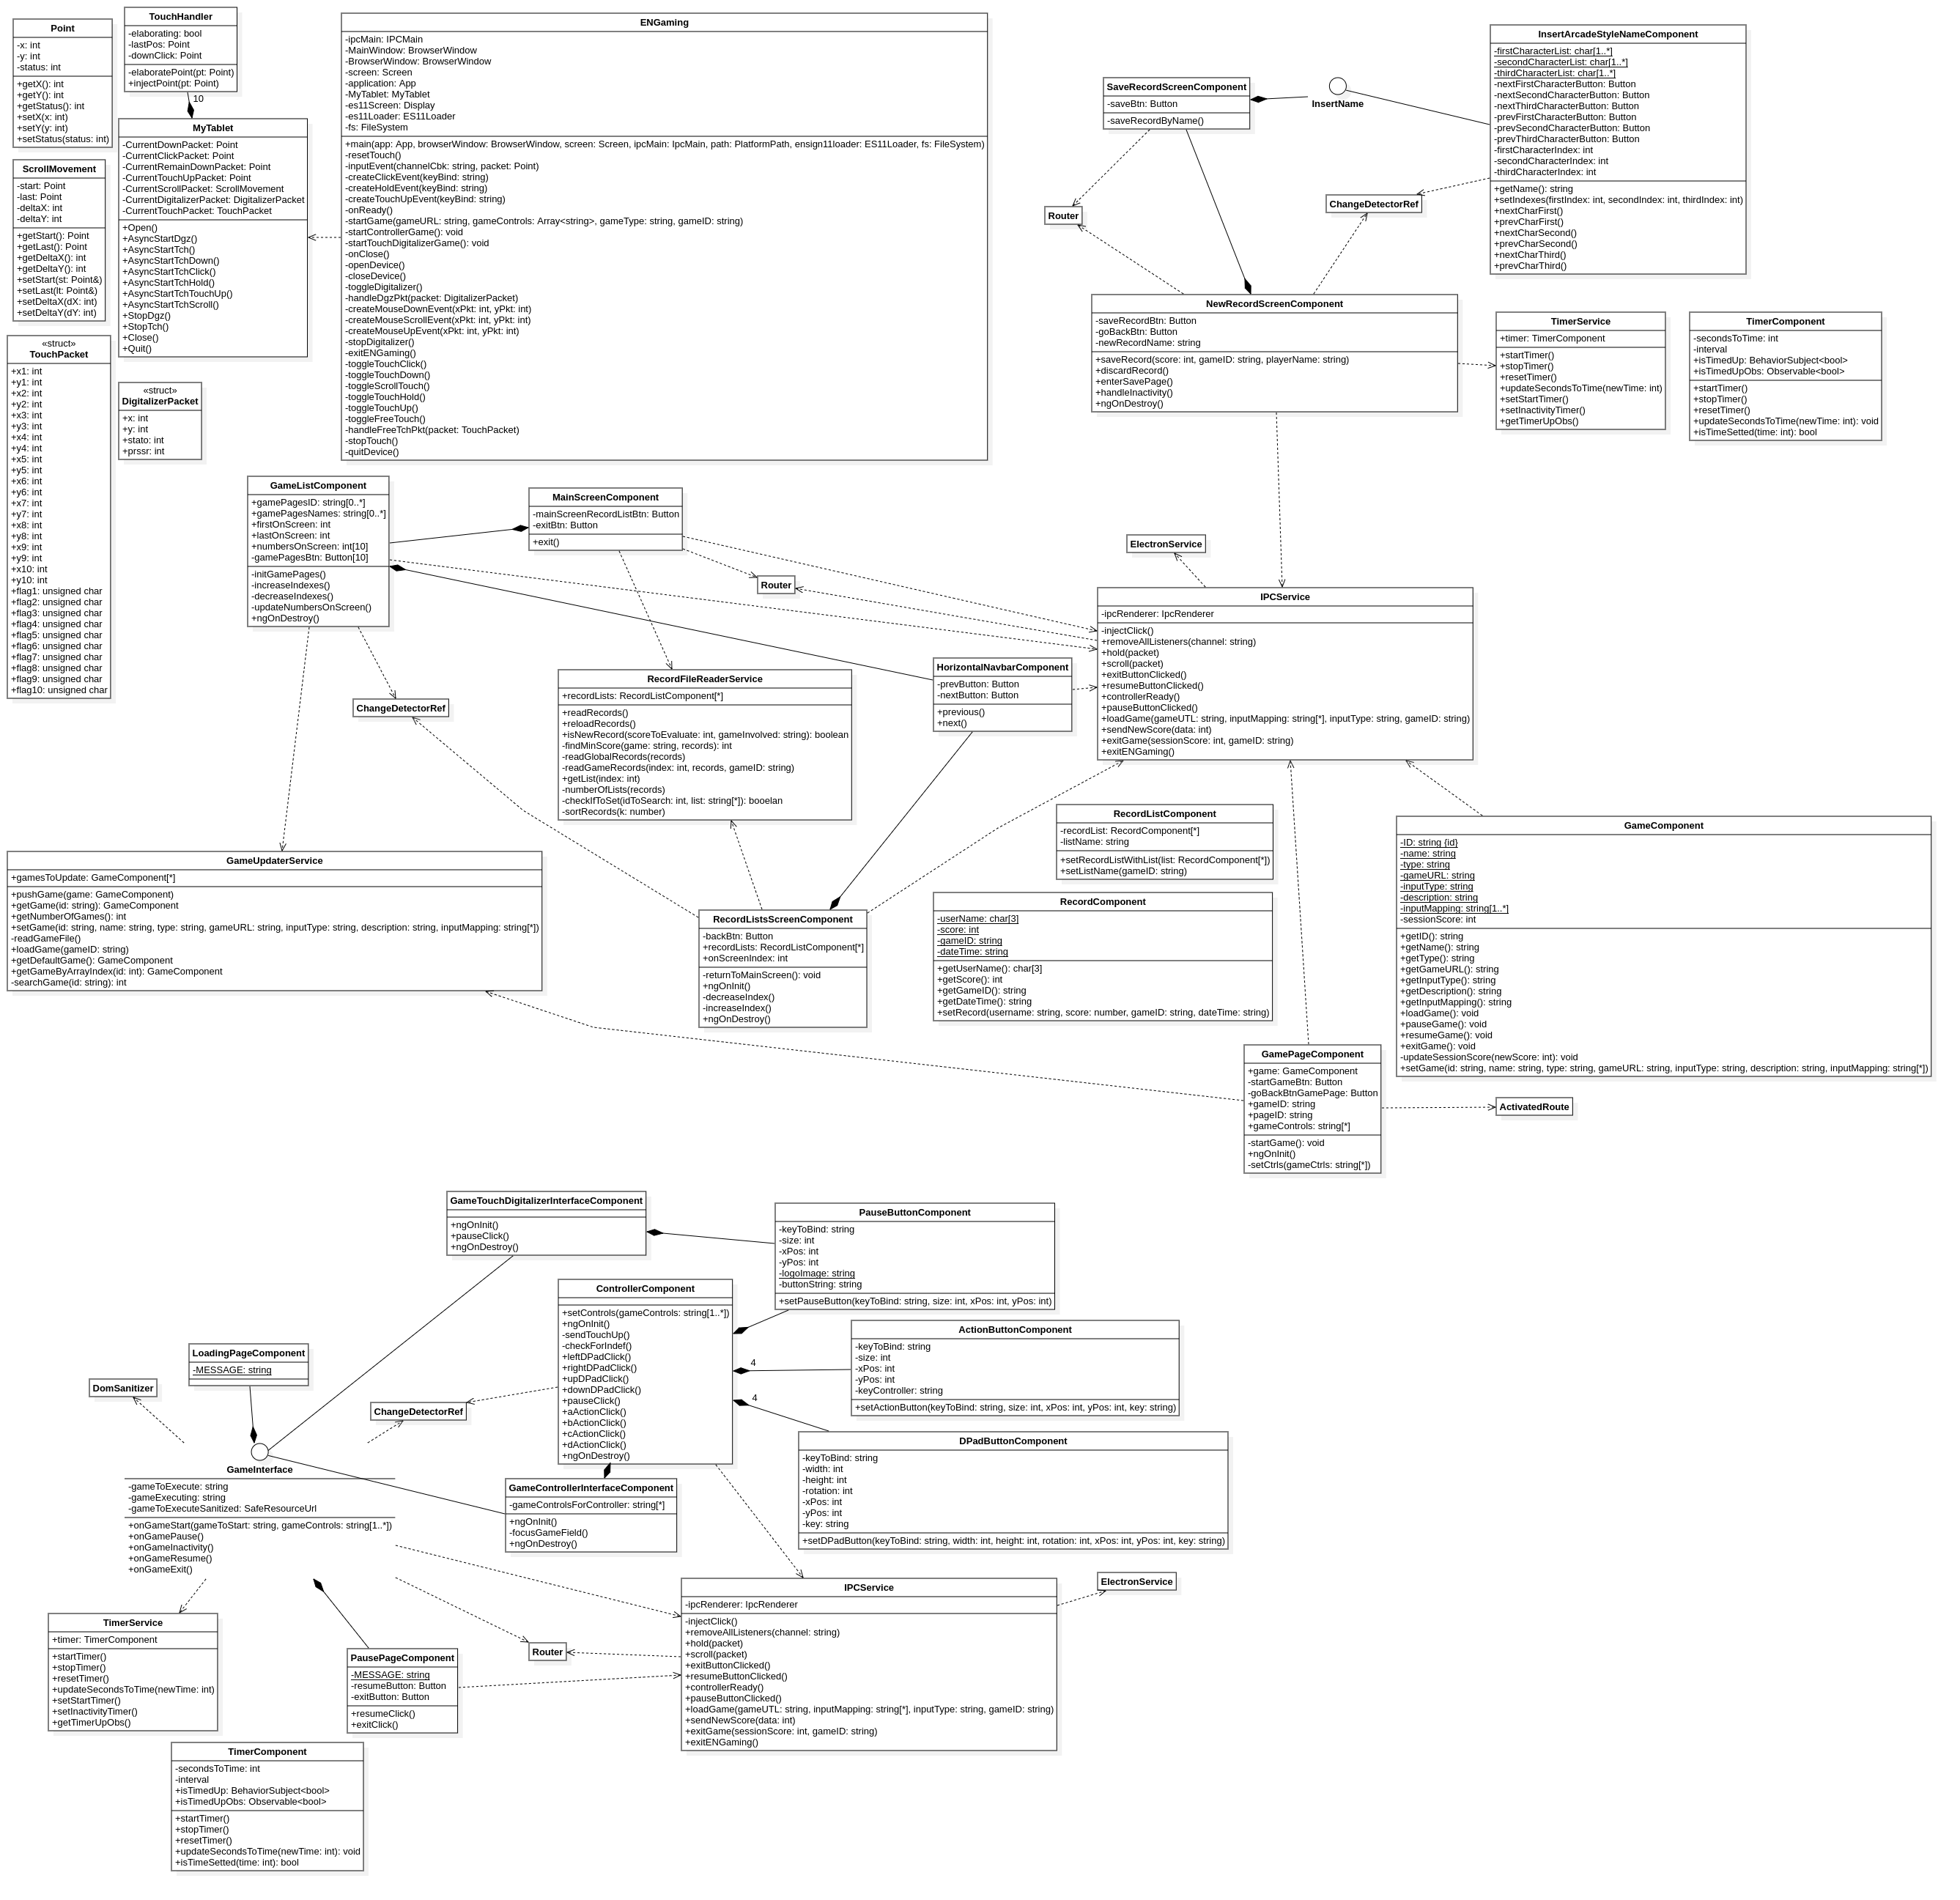
\includegraphics[width=340pt]{images/prog/ENGaming.png}
    \caption{Classe ENGaming}
    \label{fig:engaming}
\end{figure}
% immagine dettaglio ENGaming
La classe ENGaming si occupa dell'avvio dell'applicazione.\\ Sviluppata in Electron, contiene i componenti necessari per la creazione della finestra nell'ENSign 11 (Screen, BrowserWindow) e per la comunicazione con la parte in Angular (IPCMain).\\
Inoltre, contiene anche i moduli per la comunicazione con ENSign11.\\
Contiene:
\begin{itemize}
    \item i metodi per interagire con l'ENSign11: \begin{itemize}
        \item \emph{openDevice}, per aprire il device.
        \item \emph{toggleTouchClick}, per ricevere un click.
        \item \emph{toggleTouchDown}, per ricevere un down, ovvero l'evento di un dito appoggiato sullo schermo del device.
        \item \emph{toggleTouchHold}, per ricevere un hold, ovvero l'evento di un dito ancora appoggiato sullo schermo del device.
        \item \emph{toggleTouchUp}, per ricevere un touch up, ovvero l'evento di un dito sollevato dallo schermo del device.
        \item \emph{toggleScrollTouch}, per ricevere un evento di scroll, ovvero un evento di movimento di un dito sullo schermo del device.
        \item \emph{toggleFreeTouch}, per ricevere i pacchetti definiti nella struttura \emph{TouchPacket}.
        \item \emph{stopTouch}, per fermare le interazioni con lo schermo del device.
        \item \emph{toggleDigitalizer}, per ricevere i pacchetti definiti nella struttura \emph{DigitalizerPacket}.
        \item \emph{stopDigitalizer}, per fermare le interazioni con il digitalizer.
        \item \emph{closeDevice}, per chiudere il device.
        \item \emph{quitDevice}, per "liberare" il device e renderlo disponibile ad altri applicativi (o ad una nuova istanza di ENGaming).
    \end{itemize}
    \item i metodi per l'avvio dei giochi: \begin{itemize}
        \item \emph{startGame}: identifica la tipologia del gioco e lo inizializza.
        \item \emph{startControllerGame}: inizializza un gioco che richiede l'uso del controller.
        \item \emph{startTouchDigitalizerGame}: inizializza un gioco che richiede l'uso del dito o del digitalizer.
    \end{itemize}
    \item i metodi per interagire con un gioco che utilizza il controller: \begin{itemize}
        \item \emph{inputEvent}, che permette l'interazione con il controller, nell'apposito componente.
        \item \emph{createClickEvent}, che crea l'evento "click" nella pagina del gioco.
        \item \emph{createHoldEvent}, che crea l'evento "hold" nella pagina del gioco.
        \item \emph{createTouchUpEvent}, che crea l'evento "touch up" nella pagina del gioco.
    \end{itemize}
    \item i metodi per interagire con un gioco che utilizza il dito o il digitalizer: \begin{itemize}
        \item \emph{handleFreeTchPkt}: in base allo stato del pacchetto, si decide che evento sollevare.
        \item \emph{handleDgzPkt}: come per \emph{handleFreeTchPkt}, per il digitalizer.
        \item \emph{createMouseDownEvent}: crea l'evento di appoggio del dito/digitalizer nel gioco.
        \item \emph{createMouseScrollEvent}, crea l'evento di movimento del dito/digitalizer nel gioco.
        \item \emph{createMouseUpEvent}, crea l'evento di sollevamento del dito/digitalizer nel gioco.
    \end{itemize}
    \item \emph{resetTouch}: ripristina il touch del device alla fine di un gioco.
    \item \emph{exitENGaming}: chiude l'applicazione.
\end{itemize}
\newpage
\subsubsection{Schermata iniziale}
\begin{figure}[h]
    \centering
    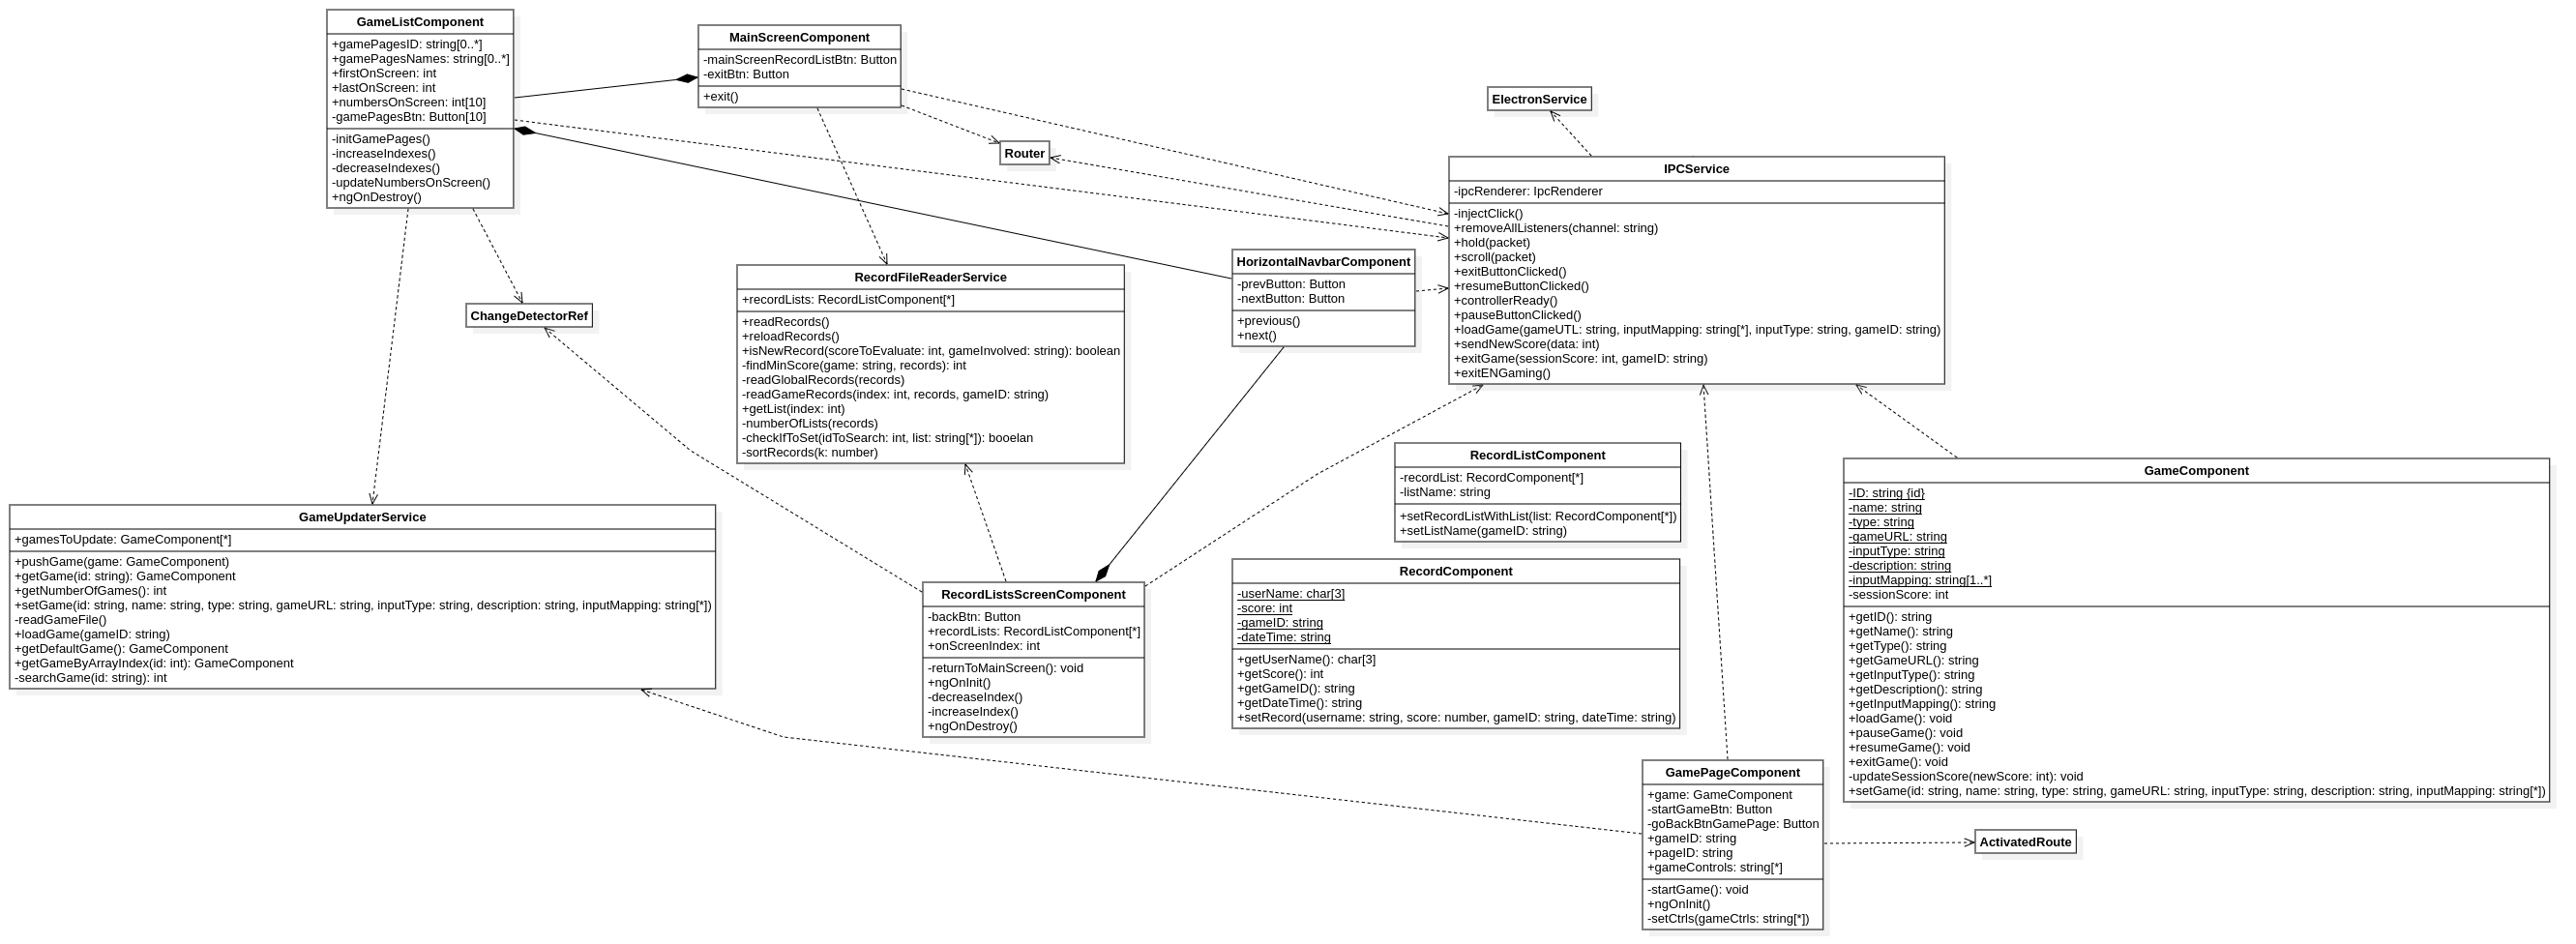
\includegraphics[width=340pt]{images/prog/MainScreen.png}
    \caption{Classi della schermata iniziale}
    \label{fig:schermataIniziale}
\end{figure}
% immagine dettaglio schermata iniziale
All'avvio dell'applicazione, la schermata iniziale presenta tre elementi:
\begin{itemize}
    \item L'elenco dei giochi disponibili, ottenuto da \emph{GameListComponent}.
    \item Il pulsante per accedere alla pagina di \emph{RecordListScreenComponent}.
    \item Il pulsante per uscire dall'applicazione.
\end{itemize}
Come si evince dal diagramma, le parti che compongono la schermata principale sono strettamente collegate tra di loro.\\
Infatti, a sua volta:
\begin{itemize}
    \item \emph{RecordListScreenComponent} è formato da almeno una \emph{RecordListComponent}, poichè la schermata ha almeno la lista globale dei record, anche se vuota. Inoltre, utilizza il \emph{HorizontalNavbarComponent} per navigare tra una lista e l'altra.
    \item \emph{RecordListComponent} contiene il nome della lista stessa e un IPCRenderer per la comunicazione con il resto dell'applicazione.\\ Ovviamente, contiene anche vari \emph{RecordComponent}, gestendosi il caso in cui non ci siano record presenti.
    \item \emph{GameListComponent} è formato sia dall' \emph{HorizontalNavbarComponent},\\ poichè gestisce la visualizzazione della lista di giochi disponibili, sia da almeno una \emph{GamePageComponent}, ossia da almeno una pagina relativa ad un gioco.
    \item Ogni \emph{GamePageComponent} è relativa ad un solo \emph{GameComponent}. Contiene sia il \emph{GameComponent}, sia i pulsanti per avviare il gioco e per tornare alla schermata principale.
\end{itemize}
\emph{GameComponent} e \emph{RecordComponent} utilizzano anche determinate proprietà, che si elencano negli appositi paragrafi.
\subsubsection{GameComponent}
\begin{figure}[h]
    \centering
    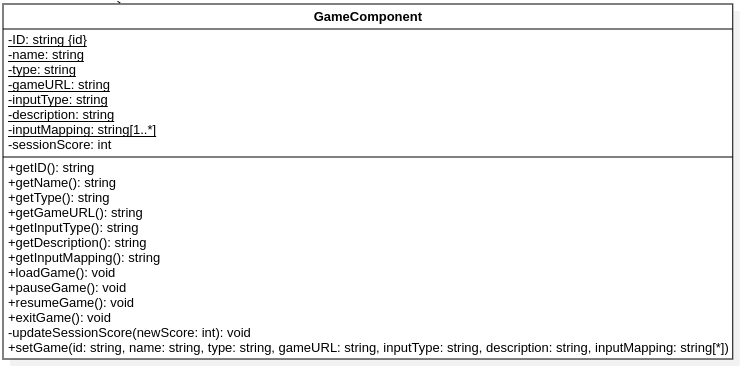
\includegraphics[width=340pt]{images/prog/Game.png}
    \caption{Dettaglio della classe GameComponent}
    \label{fig:gameComponent}
\end{figure}
% immagine dettaglio GameComponent
GameComponent rappresenta un gioco all'interno dell'applicativo. Contiene tutte le informazioni necessarie per l'avvio e il controllo dello stesso, oltre alle classice informazioni "anagrafiche".\\
Un gioco viene rappresentato come:
\begin{itemize}
    \item ID: l'identificativo del gioco, formato da una stringa.
    \item name: nome del gioco.
    \item type: la categoria del gioco.
    \item gameURL: l'indirizzo dove reperire la finestra di gioco, sia locale che remoto.
    \item inputType: la tipologia di input, tra "controller" e "touchDigit" (ovvero touch/digitalizer).
    \item description: opzionale. Descrizione del gioco, con informazioni generali in merito. Se non sono disponibili, il campo assume valore "not_available".
    \item inputMapping: la mappatura dei controlli da utilizzare per giocare.
\end{itemize}
Inoltre, contiene un gameRenderer per inviare e ricevere eventi inerenti al gioco in esecuzione, e la variabile sessionScore per registrare il punteggio di gioco più alto durante la sessione.
Infine, i giochi sono memorizzati nel file \emph{games.json}, con la struttura dell'esempio seguente:
\begin{lstlisting}[language=json,firstnumber=1]
    {"games": {
            "id": "catMario",
            "name": "Cat Mario",
            "type": "Azione",
            "gameURL": "https://www.cat-mario.com/",
            "inputType": "controller",
            "description": "Clone di Super Mario, con un gatto. Per nulla stressante!",
            "inputMapping": "["salto: bottone 1","muovi a sinistra: leva D-Pad sinistra","muovi a destra: leva D-Pad destra"]"
        },
        {
            "id": "subwaySurfers",
            "name": "Subway Surfers",
            "type": "Endless",
            "gameURL": "https://subway-surfers.me/",
            "inputType": "touchDigit",
            "description": "not_available",
            "inputMapping": "["inizia: tap","muovi a sinistra: swipe a sinistra","muovi a destra: swipe a destra","salto: swipe in alto","rotolata:swipe in basso"]"
        }
    }
\end{lstlisting}
\subsubsection{RecordComponent}
\begin{figure}[h]
    \centering
    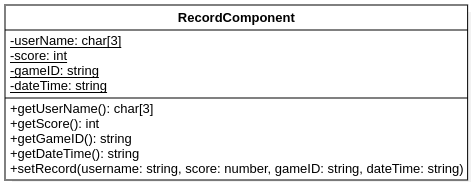
\includegraphics[width=340pt]{images/prog/Record.png}
    \caption{Dettaglio della classe RecordComponent}
    \label{fig:recordComponent}
\end{figure}
% immagine dettaglio RecordComponent
RecordComponent rappresenta un record memorizzato dall'applicativo.\\ Contiene le informazioni relative ad un punteggio, effettuato da un determinato utente in un determinato gioco.\\
Un record viene rappresentato come:
\begin{itemize}
    \item userName: il nome dell'utente che ha effettuato un record, formato da un array di tre caratteri.
    \item score: il punteggio eseguito dall'utente.
    \item gameID: l'ID del gioco dove si è effettuato il record.
    \item dateTime: la data ed ora di conseguimento del record.
\end{itemize}
Come si evince dal diagramma, non è impostato il metodo per ottenere il valore di dateTime. Questo perchè ai fini dell'applicativo non è rilevante conoscere quando è stato effettuato il record (vedasi \emph{RecordListComponent}).\\
I record sono memorizzati nel file \emph{records.json}, con la struttura dell'esempio seguente:
\begin{lstlisting}[language=json,firstnumber=1]
    {"records": {
            "userName": "AAA",
            "score": "250",
            "gameID": "dukeNukem",
            "dateTime":"2024-02-15 17:23"
        },
        {
            "userName": "RIC",
            "score": "420",
            "gameID": "angryBirds",
            "dateTime":"2024-05-19 08:23"
        }
    }
\end{lstlisting}
\subsubsection{Interfaccia di gioco}
\begin{figure}[h]
    \centering
    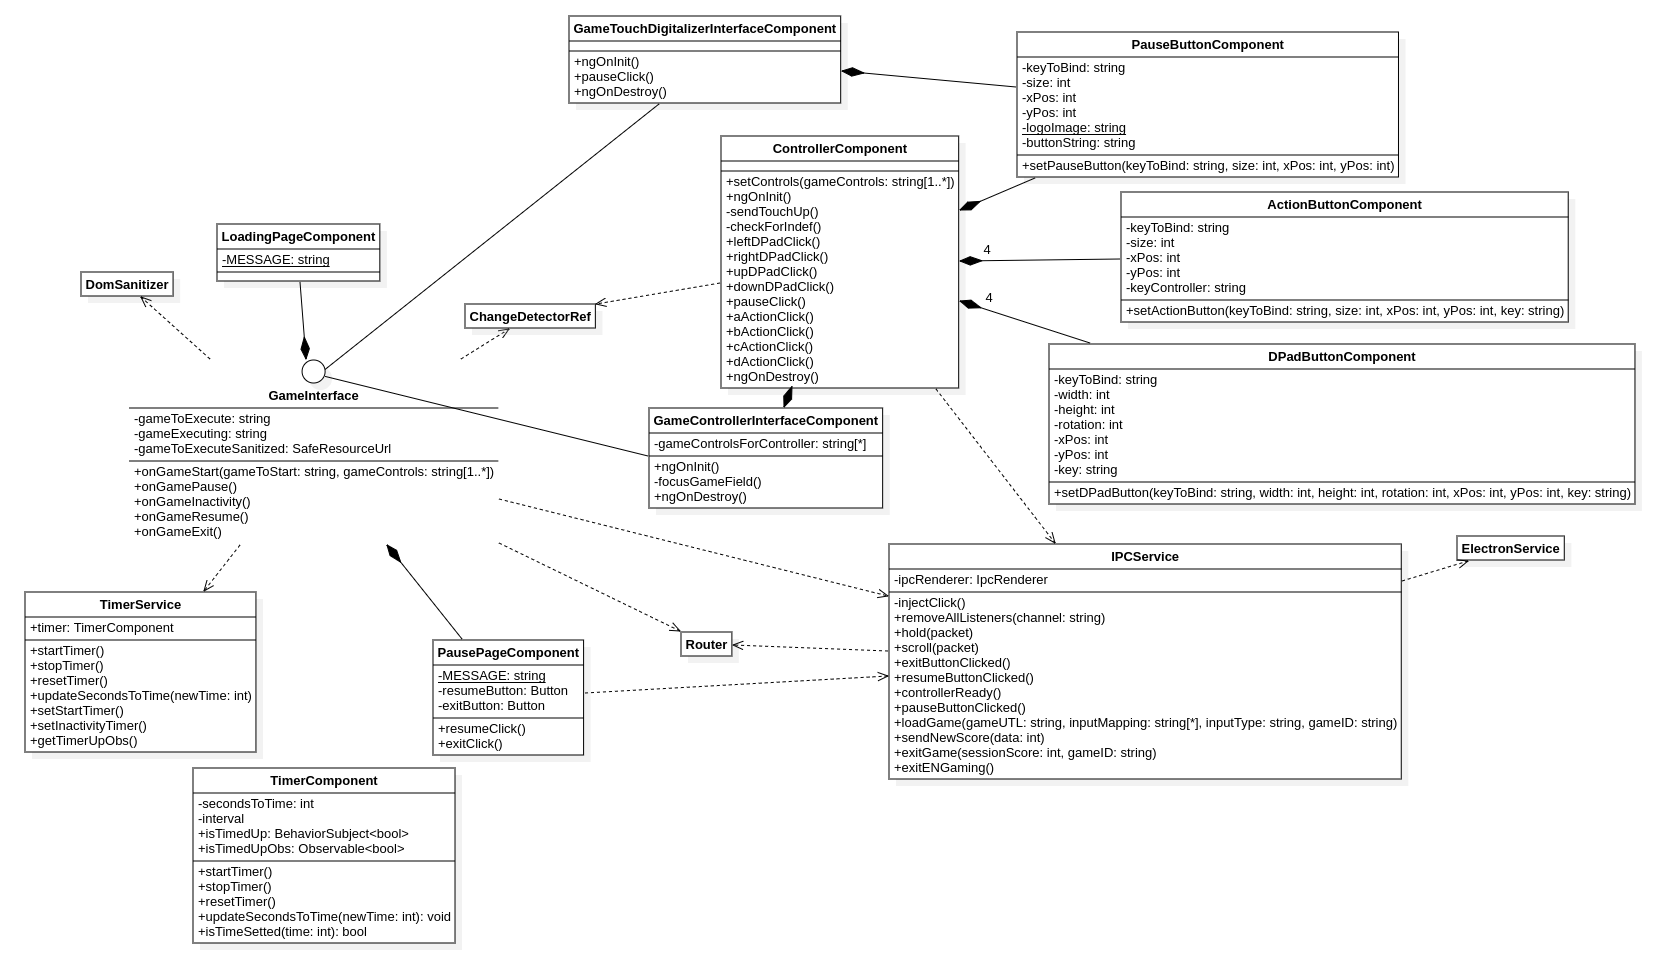
\includegraphics[width=340pt]{images/prog/GameInterface.png}
    \caption{Diagramma delle classi per l'interfaccia di gioco}
    \label{fig:gameinterface}
\end{figure}
% immagine dettaglio Interfaccia di gioco
Dovendo implementare due tipologie di gioco, dev'essere necessario poter creare due interfacce separate, che abbiano però elementi in comune.\\
Per questo motivo, viene utilizzata l'interfaccia \emph{GameInterface}, che contiene il necessario per la corretta visualizzazione del gioco.\\
In particolare, utilizza:
\begin{itemize}
    \item un \emph{TimerComponent} per la gestione della schermata di caricamento e lo stato di inattività.
    \item un \emph{LoadingPageComponent} per la visualizzazione della schermata di caricamento.
    \item un \emph{PausePageComponent} per visualizzare l'informazione dello stato di pausa del gioco, con le possibilità di riprenderlo o di uscire dallo stesso.
\end{itemize}
Questa interfaccia viene implementata da due classi: \emph{GameControllerInterfaceComponent} e \emph{GameTouchDigitalizerInterfaceComponent}.
\newpage
\subsubsubsection{GameControllerInterfaceComponent}
\emph{GameControllerInterfaceComponent} rappresenta l'interfaccia di gioco per giochi che richiedono l'utilizzo del controller.\\
Questa classe, oltre ad essere formata dagli elementi che implementa da \emph{GameInterface}, è formata da un controller. Tale controller è composto da:
\begin{itemize}
    \item 4 \emph{DPadButtonComponent}, che rappresentano i pulsanti per il movimento all'interno del gioco.
    \item 4 \emph{ActionButtonComponent}, che rappresentano i pulsanti per le azioni\\ all'interno del gioco.
    \item Un \emph{PauseButtonComponent} per mettere in pausa il gioco.
\end{itemize}
Il controller viene configurato, prima dell'avvio, secondo i comandi previsti per il singolo gioco.\\
Infine, essendo il device target posizionato in un determinato modo, è importante che il layout venga configurato in maniera da facilitarne l'utilizzo senza prendere in mano il device.\\
Un esempio è la seguente figura, dove si vede un possibile layout:
\begin{figure}[h]
    \centering
    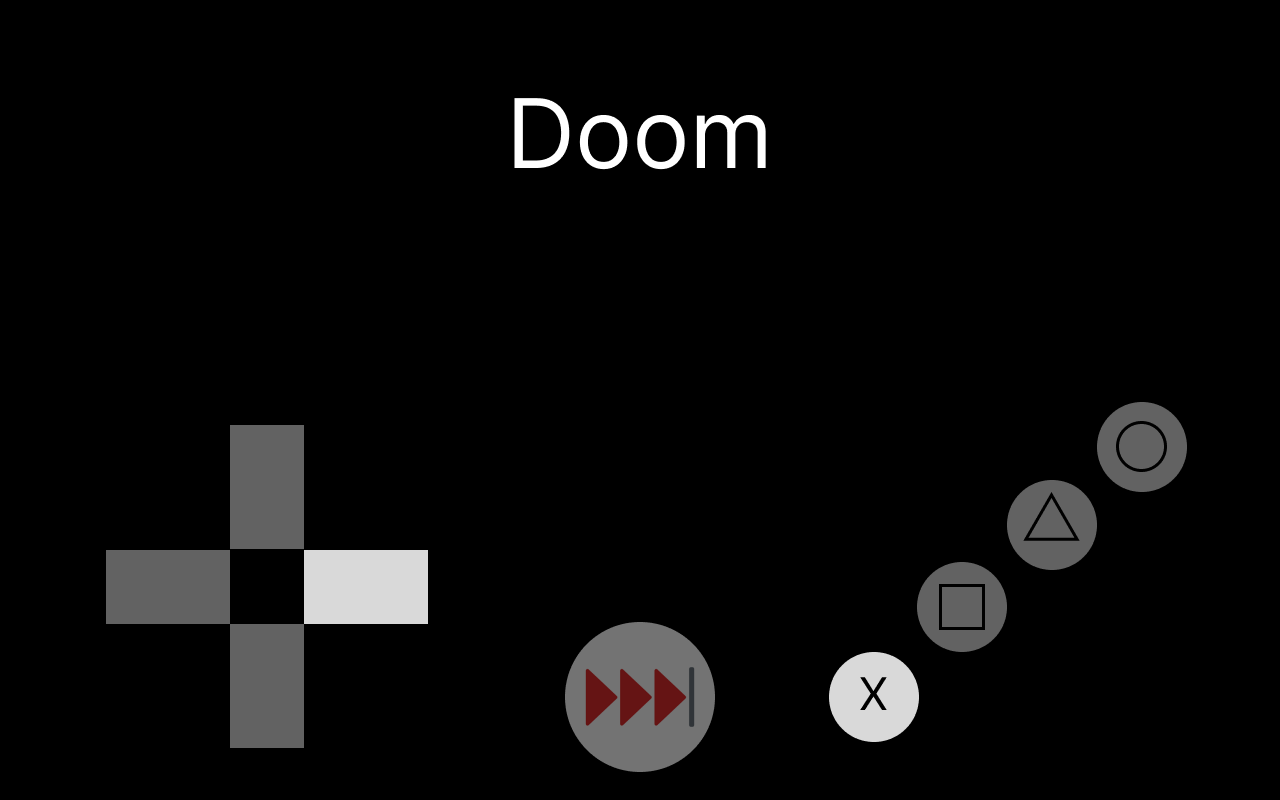
\includegraphics[width=340pt]{images/prog/ControllerMockup.png}
    \caption{Prototipo dell'interfaccia per giochi che richiedono l'uso del controller}
    \label{fig:controller}
\end{figure}
% immagine mockup controller
\subsubsubsection{GameTouchDigitalizerInterfaceComponent}
\emph{GameTouchDigitalizerInterfaceComponent} rappresenta l'interfaccia di gioco per giochi che richiedono l'utilizzo del touch, e permettono l'utilizzo del digitalizer.\\
Questa classe, oltre ad essere formata dagli elementi che implementa da \emph{GameInterface}, è formata da un \emph{PauseButtonComponent} per mettere in pausa il gioco.\\
Il \emph{PauseButtonComponent} viene configurato, prima dell'avvio, secondo i comandi previsti per il singolo gioco.\\
Infine, essendo il device target posizionato in un determinato modo, è importante che il \emph{PauseButtonComponent} venga messo in modo da invadere il meno possibile lo spazio di gioco.\\
Un esempio è la seguente figura, dove si vede una possibile collocazione:
\begin{figure}[h]
    \centering
    
\includegraphics[width=340pt]{images/prog/TouchDigitMockup.png}
    \caption{Prototipo dell'interfaccia per giochi che richiedono l'uso di touch/digitalizer}
    \label{fig:touchDigit}
\end{figure}
% immagine mockup touch/digitalizer
\newpage
\subsubsection{Schermata di salvataggio record}
\begin{figure}[h]
    \centering
    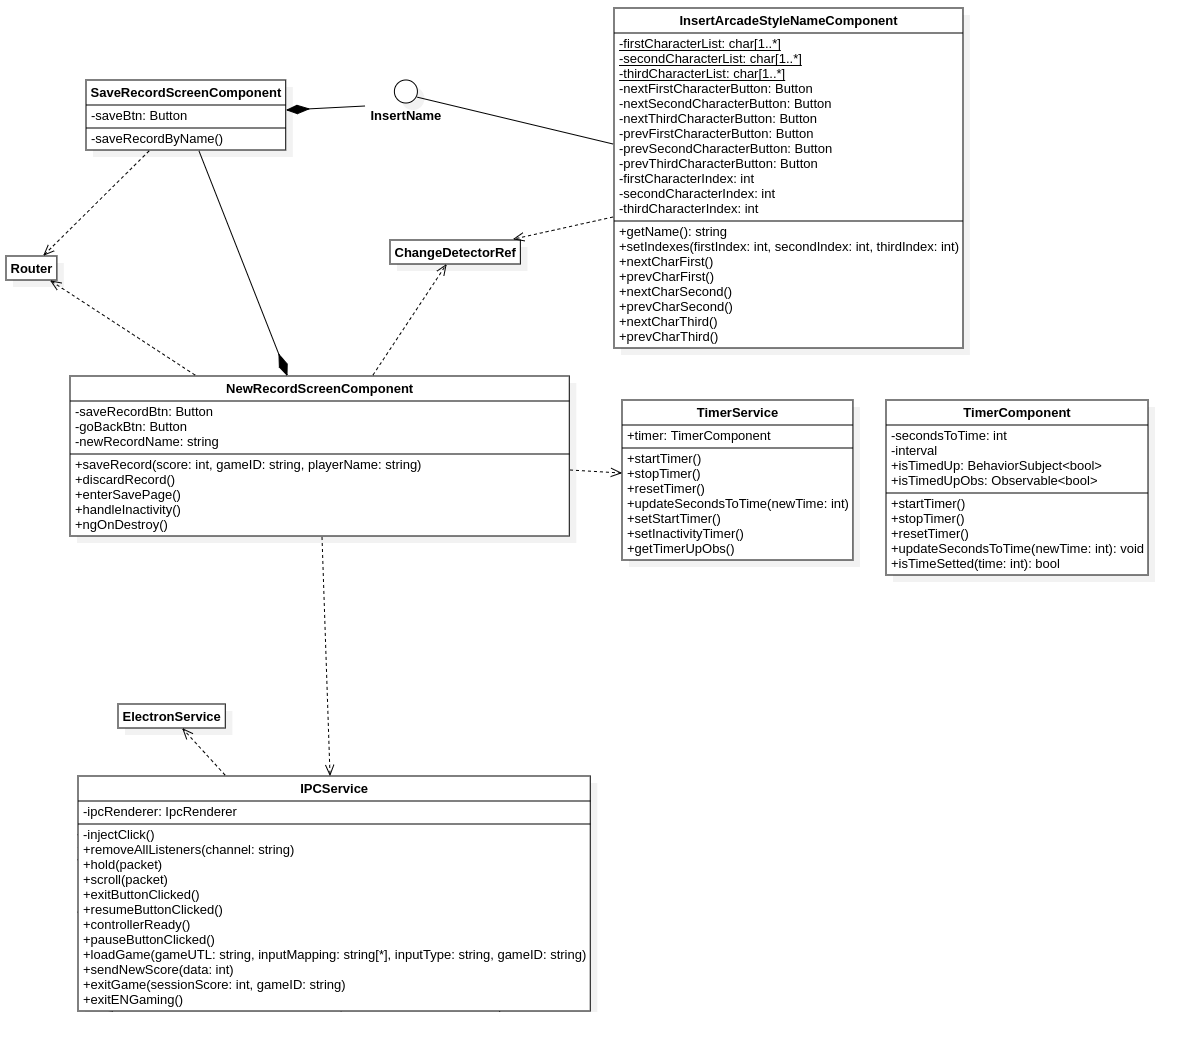
\includegraphics[width=340pt]{images/prog/NewRecord.png}
    \caption{Diagramma delle classi per il salvataggio dei record}
    \label{fig:attore}
\end{figure}
% immagine dettaglio salvataggio record
Alla notifica di un nuovo record, viene visualizzata la pagina \emph{NewRecordScreenComponent}, dove viene chiesto all'utente se desidera salvare il record appena effettuato o non salvarlo.\\
Nel caso di salvataggio del record, si passa alla pagina \emph{SaveRecordScreenComponent}, che si occupa di ricevere il nome dell'utente. Per far ciò, si avvale della classe \emph{InsertArcadeStyleNameComponent}.\\
Tale classe, che implementa l'interfaccia \emph{InsertName}, prevede l'inserimento dei tre caratteri che compongono il nome utente scegliendo tra i caratteri disponibili, utilizzando gli appositi bottoni.\\
\emph{SaveRecordScreenComponent} inoltre utilizza anche \emph{TimerComponent} per la gestione dell'inattività in quella determinata schermata.
\subsubsection{TimerComponent}
\begin{figure}[h]
    \centering
    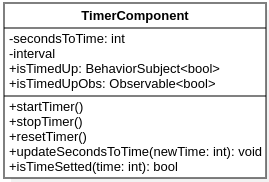
\includegraphics[width=200pt]{images/prog/TimerComponent.png}
    \caption{Dettaglio della classe TimerComponent}
    \label{fig:timer}
\end{figure}
% immagine dettaglio TimerComponent
\emph{TimerComponent} si occupa della gestione del tempo. Il suo scopo è, dato un tempo espresso con un valore decimale, di iniziare il conteggio, e notificare quando il tempo ha raggiunto la fine.\\
Per far questo, calcola la data di scadenza del timer partendo da quella attuale, notificando quando entrambe combaciano.
\subsubsection{Gestione ENSign11}
\begin{figure}[h]
    \centering
    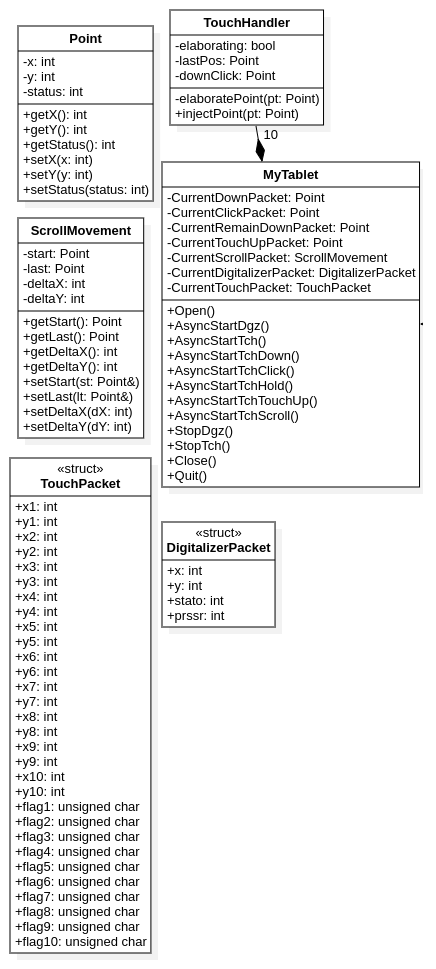
\includegraphics[width=340pt]{images/prog/ENS11.png}
    \caption{Diagramma per la gestione dell'input da ENSign11}
    \label{fig:es11}
\end{figure}
% immagine dettaglio gestione ENSign11
Per il recupero dell'input dal device ENSign11, l'applicativo si serve di tre elementi:
\begin{itemize}
    \item LibENSign11: driver del device che permette l'utilizzo del sistema touch e del digitalizer.
    \item MyTablet: classe che si occupa dell'apertura e della chiusura del tablet, oltre all'apertura e chiusura sia del sistema touch sia del digitalizer.
    \item TouchHandler: classe che invia alla parte Electron-Angular gli eventi. Tra gli eventi ci sono: \begin{itemize}
        \item l'invio di un tocco semplice, restituendo le coordinate x e y del tocco.
        \item l'invio di un tocco prolungato, sempre restituendo le coordinate x e y del tocco.
        \item l'invio di uno swipe, restituendo le coordinate x e y inziali e i delta, ovvero le differenze di coordinate, di x e y. 
    \end{itemize}
\end{itemize}
\subsection{Struttura dei file utilizzati}